\documentclass[%
 reprint,
%superscriptaddress,
%groupedaddress,
%unsortedaddress,
%runinaddress,
%frontmatterverbose, 
%preprint,
%preprintnumbers,
%nofootinbib,
%nobibnotes,
%bibnotes,
 amsmath,amssymb,
 aps,
%pra,
%prb,
%rmp,
%prstab,
%prstper,
%floatfix,
]{revtex4-1}

\usepackage{graphicx}% Include figure files
\usepackage{dcolumn}% Align table columns on decimal point
\usepackage{bm}% bold math
\usepackage{physics}
\usepackage{booktabs}
\usepackage{xcolor}

\begin{document}

\preprint{APS/123-QED}

\title{Physics Informed Deep Operator Networks for Neutron Transport}

\author{William Eivik Olsen}
 \altaffiliation[Also at ]{Department of Physics, University of Oslo.}
\affiliation{Institute for Energy Technology}

\date{\today}

\begin{abstract}
An article usually includes an abstract, a concise summary of the work
covered at length in the main body of the article. 
\end{abstract}

\maketitle

\section{Introduction}

Global climate mitigation targets motivate the rapid expansion of low-carbon energy sources, and technological advances have renewed interest in
nuclear energy as a reliable, compact, and dispatchable option. Small Modular Reactors (SMRs), typically up to 300~MW(e) per unit, promise factory
fabrication and modular deployment \cite{IAEA_2024_SMR}. Within this landscape, microreactors at up to roughly 20~MW(e) have emerged as particularly
attractive for transportable, remote, and mobile applications, enabling reliable power in settings where conventional infrastructure is limited
\cite{black2023prospects}.

Maritime propulsion has become a prominent candidate for such deployment. Shipping is responsible for about three percent of global greenhouse gas
emissions today and could rise substantially without decisive countermeasures. The NuProShip project \cite{nuproship}, funded by the Research
Council of Norway, surveyed more than eighty reactor concepts and identified three leading candidates for ship integration: a helium gas–cooled
microreactor developed by Ultra Safe Nuclear Corporation, a molten-salt SMR by Kairos Power, and a lead-cooled SMR by Blykalla. While these
technologies show promise, NuProShip highlights crew availability and cost—especially the need for highly trained nuclear operators—as a
principal barrier to adoption. This challenge extends beyond maritime settings to the broader class of remote and mobile applications that
motivate microreactors in the first place.

To mitigate this challenge, the development of digital twin technology for microreactors has been suggested \cite{MAGNET}. A digital twin is a
digital replica of an operating asset that can receive data from live sensors and provide physics modeling and simulation of the asset. In the
nuclear context, a complete physics simulation should include the neutronics of the core, thermal-hydraulics and radiation transport
\cite{DT2024review}. An additional advantage of creating a digital twin is the ability to perform multi-physics simulations of the reactor in
the approval phase. For this reason, digital twins for maritime nuclear propulsion has gained the attention of Det Norske Veritas
(DNV), who recently initiated the research project MONS (Model-based Nuclear Safety) to investigate model based safety assessments of maritime
nuclear vessels using multi-physics simulations. This paper is a contribution to the MONS project.

The heart of such a multi-physics model is the simulation of the reactor core itself – specifically, simulating the neutron transport and the fission
chain reaction from which the core releases energy. The neutron transport equation (NTE) is notoriously difficult to solve. Traditional solution methods
can be divided into \textit{Deterministic methods}, in which simplifying assumptions are used to approximate the NTE, and \textit{Monte Carlo methods},
in which the NTE is simulated using statistical methods. Both methods are able to provide solutions of satisfying accuracy. However, a digital twin
should be able to simulate the reactor in real-time \cite{kochunas2021digital}. Deterministic and Monte Carlo methods both suffer from high
computational costs, and are unable to solve the NTE in real-time \cite{SHEN2022108861, ZHOU2024110759, sahadath2026characterization}.

The advance of machine learning methods has sparked interest in applying them to enable fast solutions of the NTE. Among them is Sahadath et al.
\cite{sahadath2026characterization}, who investigated a DeepONet trained on neutron transport of a 1D slab. In this paper, we will investigate
the performance of a \textit{Physics Informed DeepONet}, first introduced by \cite{wang2021learning}. We will evaluate its performance on the same
1D problem and compare it to that of Sahadath et al.

Such a 1D model is too simple to represent the complete reactor to be considered in the MONS project. The model developed in this paper will
serve as the first step towards a complete 3D reactor model.

\section{Theory}

\subsection{The Neutron Transport Equation}

The key problem of reactor physics is the Neutron Transport Equation (NTE). It is given by
\begin{align}
\frac{1}{v} &\frac{\partial \psi}{\partial t} + \hat{\Omega}\cdot\nabla\psi + \Sigma_t\,\psi(\mathbf{r},\hat{\Omega},E,t) = \nonumber \\
     &\int_{4\pi}\int_0^\infty \Sigma_s(\mathbf{r},\hat{\Omega}'\to\hat{\Omega},E'\to E)\,\psi(\mathbf{r},\hat{\Omega}',E',t)\,dE'\,d\Omega' \\ \nonumber
     &+ \frac{\chi(E)}{4\pi}\int_{4\pi}\int_0^\infty \nu\Sigma_f(\mathbf{r},E')\,\psi(\mathbf{r},\hat{\Omega}',E',t)\,dE'\,d\Omega' \\ \nonumber
     &+ S_{\text{ext}}(\mathbf{r},\hat{\Omega},E,t),
\end{align}
where $\psi(\mathbf{r},\hat{\Omega},E,t)$ is the angular neutron flux at position $\mathbf{r}$, travelling in direction $\hat{\Omega}$, with
energy $E$, at time $t$. The quantity $v$ is the neutron speed corresponding to energy $E$, so that
$\tfrac{1}{v}\tfrac{\partial \psi}{\partial t}$ represents the time rate of change of the neutron population.

The term $\hat{\Omega}\cdot\nabla\psi$ is the streaming (leakage) term, accounting for neutrons moving through the spatial domain.
The macroscopic total cross section $\Sigma_t$ governs the loss of neutrons from the phase-space element due to all interactions
(absorption plus scattering), so $\Sigma_t\,\psi$ is the total collision (removal) term.

On the right-hand side, $\Sigma_s(\mathbf{r},\hat{\Omega}'\to\hat{\Omega},E'\to E)$ is the double-differential macroscopic scattering cross
section, describing neutrons that scatter from direction $\hat{\Omega}'$ and energy $E'$ into direction $\hat{\Omega}$ and energy $E$.
The integral over all incoming directions $\hat{\Omega}'$ (over the unit sphere, $4\pi$ steradians) and all incoming energies $E'$ gives
the in-scattering source.

The second term on the right side is the fission source term. The integral of the fission cross section $\Sigma_f$ weighted by the neutron flux
$\psi$ and the neutrons released per fission $\nu$ gives the total number of neutrons which are emitted isotropically. The integral is multiplied
by the fission spectrum $\chi(E)$, such that the final result is the number of fission neutrons at energy $E$.

Finally, $S(\mathbf{r},\hat{\Omega},E,t)$ is the external neutron source term.

The NTE describes the interactions of neutrons in the reactor and, importantly, the fissions they cause along with the new neutrons
released from fission. A nuclear reactor is a controlled fission chain reaction, with the goal of producing as many new neutrons from fissions
as the number lost through absorption or leakage. To model this, it is therefore necessary to solve the NTE.

The NTE is traditionally solved using either Monte Carlo methods or Deterministic methods. Both are computationally expensive, which is what
motivates us to introduce machine learning methods to approximate solutions. However, in order to train a machine learning model, we must have
training data. This can be generated by solving the NTE with traditional methods. Given the computational expense of traditional methods, we
might face a challenge to generate enough training data for our model. This motivates the use of \textit{Physics-Informed} training, where we
introduce an additional loss term that represents the governing differential equation of the problem.

\subsection{Machine Learning Methods}

\subsubsection{Physics-Informed Neural Networks}

\begin{figure}
    \centering
    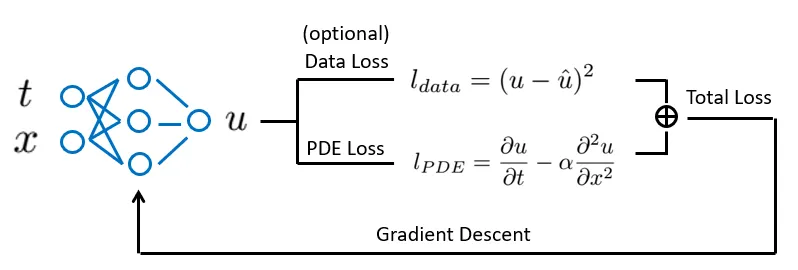
\includegraphics[width=\linewidth]{figures/PINN.png}
    \caption{Illustration of a PINN. Adapted from \cite{deeponet_medium_2023}.}
    \label{fig: PINN}
\end{figure}

A Physics-Informed Neural Network (PINN) is a type of deep learning model designed to solve problems governed by physical laws,
specifically those described by partial differential equations (PDEs) \cite{raissi2019physics}. It uses a standard neural network to approximate
the unknown solution as a function of input variables. The key idea is that the network is trained not only to match available data points, but
also to satisfy the governing PDE itself within the domain, as illustrated in Figure \ref{fig: PINN}. This \say{physics-informed} constraint is
incorporated into the training process by calculating the PDE residual using automatic differentiation and minimizing it alongside the standard
loss function.

An advantage of PINNs in neutronics is their ability to perform fast computations. While the training process can require significant
computational resources, once trained, the model can make predictions quickly. PINNs have been studied by several authors in the context of
neutronics. Prantikos et al. \cite{prantikos2022physics} implemented a PINN model trained on the point kinetics equations and tested its
predictions using experimental data from Purdue University Reactor Number One (PUR-1). More recently, studies have explored PINNs trained with
the neutron diffusion equation \cite{elhareef2023physics} and the neutron transport equation \cite{xie2024boundary}.

One disadvantage with PINNs is that they require retraining for new input boundary/initial conditions \cite{sahadath2026characterization}. This
is challenging for the maritime settings, where initial and boundary conditions are expected to vary dynamically.

\subsubsection{Deep Operator Networks}

The disadvantage we discussed with PINNs are shared with most traditional machine learning methods, as they  learn pointwise mapping between
input-output data pairs. Deep operator networks, on the other hand, learn mappings between entire input and output function spaces. DeepONets
treat inputs and outputs as functions, and aim to learn the solution operator that maps initial or boundary condition functions to corresponding
solution functions \cite{sahadath2026characterization}. This framework of learning the function mapping allows them to generalize to previously
unseen conditions without the need for retraining. A DeepONet can therefore act as a sufficient surrogate model for the neutron transport
equation, delivering accurate predictions for a wide range of scenarios while maintaining high generalization performance.

A DeepONet consists of two neural networks:
\begin{itemize}
    \item A TrunkNet that processes evaluation points, such as time or spatial coordinates.
    \item A BranchNet that encodes discretized condition functions, such as initial and boundary conditions.
\end{itemize}
The final output is obtained through the dot product of the output of these two networks. An illustration of the DeepONet architecture is shown
in figure \ref{fig: DeepONet}.

\begin{figure}
    \centering
    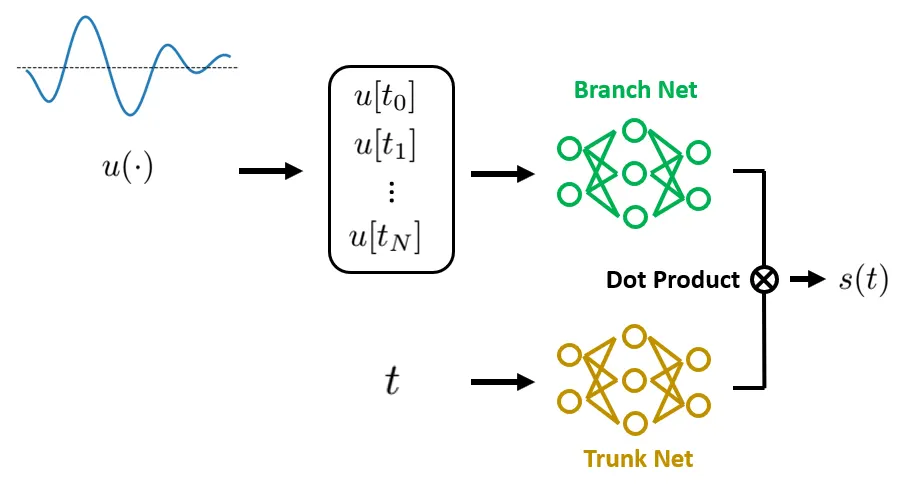
\includegraphics[width=\linewidth]{figures/DeepONet.png}
    \caption{Illustration of a Deep Operator Network. Adapted from \cite{deeponet_medium_2023}.}
    \label{fig: DeepONet}
\end{figure}

Consider an input function $u(x)$ that can be sampled at a set of discrete positions $\{x_1, x_2, ..., x_m\}$ in the domain $D_x$ as
$[u(x_1), u(x_2, ..., u(x_m)]$. Given an operator $G$ that acts on $u(x)$, $G(u)$ represents the resulting output function in domain $D_y$.
Note that the domains $D_x$ and $D_y$ are not necessarily the same and can be entirely different. Within the domain of $G(u)$, the real value at
any sampling point $y_i$ is expressed as $G(u)(y_i)$. From the generalized universal approximation theorem for operators, for any $\epsilon > 0$,
there exists positive integers $n,p$ and continuous vector functions
$\mathbf{g}: \mathbb{R}^n \to \mathbb{R}^p$ and $\mathbf{f}: \mathbb{R}^d \to \mathbb{R}^p$ such that
\begin{equation}
    |G(u)(y_i) - \langle g(u(x_1), ..., u(x_m)), f(y_i) \rangle| < \epsilon,
\end{equation}
where $\langle \cdot, \cdot \rangle$ denotes the dot product defined in $\mathbb{R}^p$, and the functions $g$ and $f$ can be represented by any
neural networks.

The approximation of $g(u(x_1), ..., u(x_m))$ is made by the BranchNet. This is done by mapping the input $[u(x_1), u(x_2, ..., u(x_m)]$ to a
vector $\mathbf{b_N} = [b_1, b_2, ..., b_p]$. The TrunkNet takes an evaluation point $y_i$ from the domain of the target operator $G(u)$ and
outputs a vector $\mathbf{t_N} = [t_1(y_i), t_2(y_i), ..., t_p(y_i)]$. Finally, the output is computed by
\begin{equation}
    G(u)(y_i) \approx \sum_{k=1}^p b_k(u(x_1), ... u(x_m)) t_k(y_i).
\end{equation}

The challenge faced by DeepONets is their requirement of large annotated datasets consisting of input-output observations. Another worry for our
usecase is the model's ability to extrapolate: If the reactor enters a state significantly outside the training distribution, the DeepONet
predictions can become unphysical.

\subsubsection{Physics-Informed DeepONets}

\begin{figure}
    \centering
    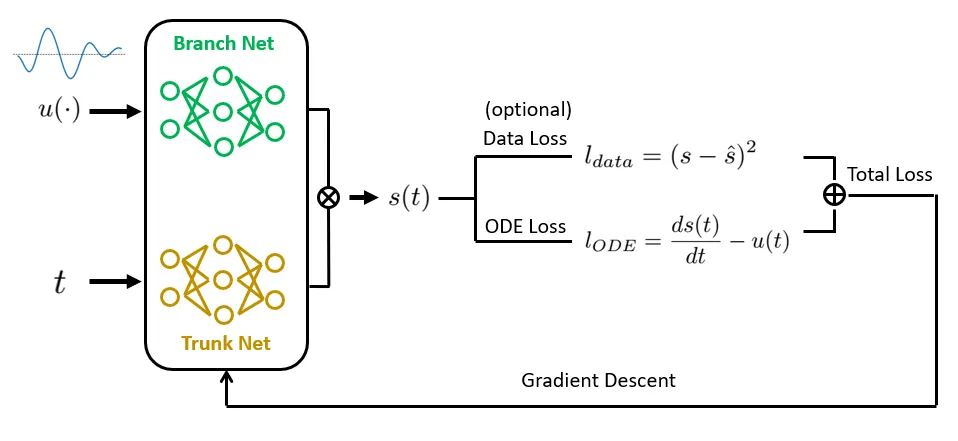
\includegraphics[width=\linewidth]{figures/PI DeepONet.png}
    \caption{Illustration of a Physics-Informed DeepONet. Adapted from \cite{deeponet_medium_2023}.}
    \label{fig: PI DeepONet}
\end{figure}

We have so far introduced PINNs and DeepONets. Both have strengths that make them suitable for solving differential equations in physics, but, as
we have seen, each of them have their drawbacks:
\begin{itemize}
    \item PINNs require retraining for every new initial and boundary condition. This is problematic for the maritime case, where we expect the
    conditions to vary dynamically.
    \item DeepONets require large annotated datasets of input-output observations, which for our case means running a large amount of Monte Carlo
    simulations of the reactor design we wish to model.
\end{itemize}
A promising method to circumvent this issue is to combine these two methods into a single framework: A Physics-Informed DeepONet.
The architecture is visualized in figure \ref{fig: PI DeepONet}. In addition to the Branch and Trunk net, the model incorporates the governing
differential equation in its loss function. The architecture was first suggested by \cite{wang2021learning}, who demonstrated its effectiveness
on various types of PDEs, including a diffusion model.

The framework is able to combine the advantages of PINNs and DeepONets: They keep the low-data requirement of the PINN methods while being able
to generalize like a DeepONet. The physics constraint makes the model more robust to handle inputs outside the training distribution.
For these reasons, we believe Physics-Informed DeepONets to be the most promising architecture for our usecase.

\section{Problem Statement}

For this paper, we will consider the NTE for a simple 1D slab geometry. As we will see, this simplifies the NTE and allows us to easily
generate a training dataset without using Monte Carlo or deterministic approximations. The performance of a DeepONet on this problem has been
studied by \cite{sahadath2026characterization}. We will use this model as a benchmark and develop our own Physics-Informed DeepONet model on
the same problem to compare their performances.

For this specific problem, physics-informed training is not strictly necessary, since we easily
can generate training data. However, the question we wish to answer in this study is \textit{to which extent physics-informed training can replace labelled
training}. This will serve as valuable insight for our future efforts of training models for more complicated 2D or 3D problems, where training
data will be scarcer due to the necessity of using Monte Carlo or Deterministic methods for training data generation.

\section{Method}

\subsection{Neutron Transport Problem}

\begin{figure}
    \centering
    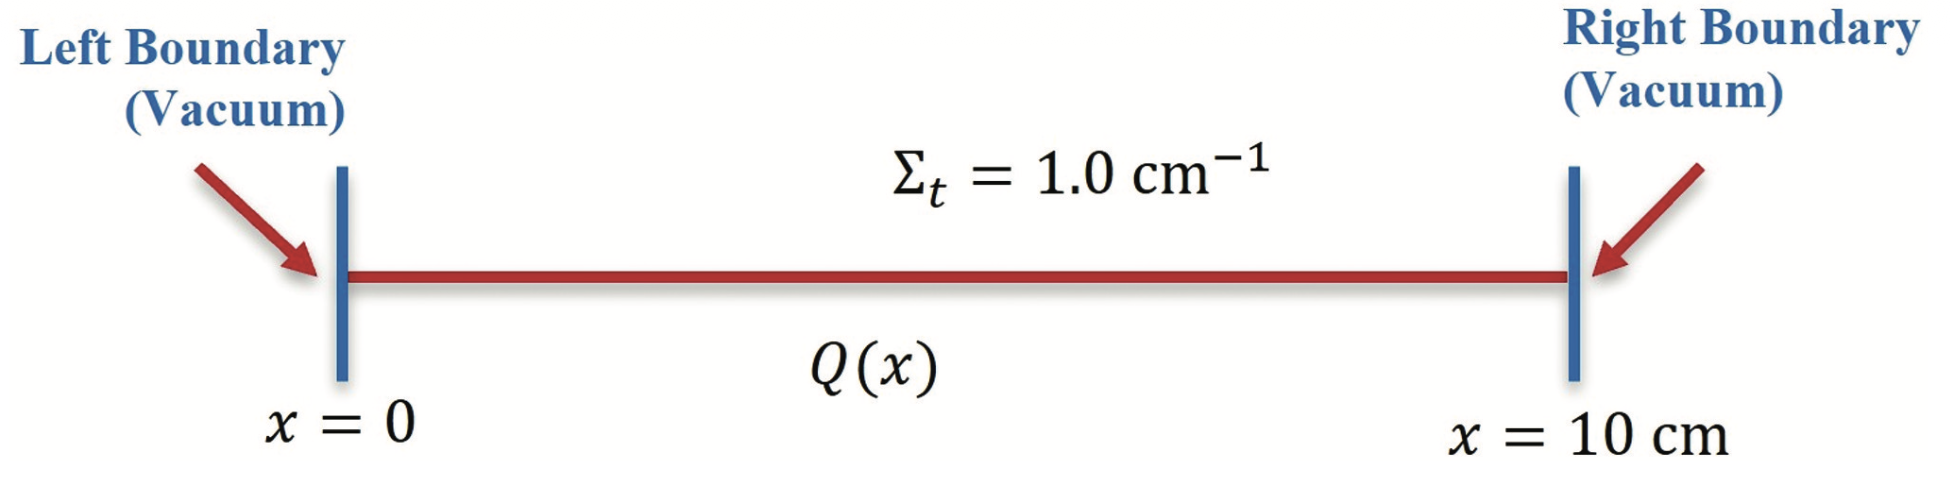
\includegraphics[width=\linewidth]{figures/1D Slab.png}
    \caption{Illustration of the 1D slab geometry. Adapted from \cite{sahadath2026characterization}.}
    \label{fig: 1D Slab}
\end{figure}

We adapt the problem from Sahadath et al. \cite{sahadath2026characterization}. The geometry is a 1D slab with a length of 10 cm,
spatially uniform cross sections and zero incoming current boundary conditions imposed at both ends. The geometry is illustrated
in Figure \ref{fig: 1D Slab}. The total cross section is assumed to be 1.0 cm$^{-1}$, while the absorption and scattering
cross section depend on the scenario considered.

The steady-state one-group NTE for this 1D slab is given by
\begin{align}
\mu \frac{\partial \psi(x, \mu)}{\partial x}
&+ \Sigma_t \, \psi(x, \mu) \nonumber \\
&= \int_{-1}^{1} \tfrac{1}{2} \left[ \Sigma_{s0} + 3 \mu \mu' \Sigma_{s1} \right]
  \psi(x, \mu') \, d\mu' \nonumber \\
&\quad + \frac{Q(x)}{2}, \nonumber \\
& \quad 0 < x < X, \quad -1 \leq \mu \leq 1 \nonumber \\
\psi(0, \mu) &= 0, \quad 0 \leq \mu \leq 1 \nonumber \\
\psi(X, \mu) &= 0, \quad -1 \leq \mu \leq 0 \label{eq: 1D NTE}
\end{align}
Here $\psi(x, \mu)$ is the angular flux at position $x$ along the slab and direction cosine $\mu$, where $\mu$ denotes the cosine of the angle
between the neutron's direction of travel and the $x$-axis. The total macroscopic cross section is $\Sigma_t$, while $\Sigma_{s0}$ and
$\Sigma_{s1}$ are the zeroth and first Legendre moments of the differential scattering cross section, respectively, with $\Sigma_{s1}$
accounting for linearly anisotropic scattering. The external neutron source distribution is denoted $Q(x)$, and $X$ is the slab length. The
boundary conditions correspond to vacuum (zero incoming current) at both ends of the slab: no neutrons enter from the left at $x = 0$ for
forward-traveling directions ($\mu > 0$), and none enter from the right at $x = X$ for backward-traveling directions ($\mu < 0$).

The angular flux $\psi(x, \mu)$ can be integrated over the angular variable $\mu$ to obtain the \textit{scalar flux} $\varphi_0(x)$,
\begin{equation} \label{eq: Scalar flux}
    \varphi_0(x) = \int_{-1}^1 \psi(x, \mu) \dd{x}.
\end{equation}
By taking the integral of the angular flux weighted by the angular variable $\mu$, the \textit{scalar current} $\varphi_1(x)$ is obtained,
\begin{equation} \label{eq: Scalar current}
    \varphi_1(x) = \int_{-1}^1 \mu \psi(x, \mu) \dd{x}.
\end{equation}

\subsection{Data Generation}

In the paper by Sahadath et al, a set of source distributions $Q(x)$ were prepared, and the 1D NTE was solved numerically for each of them to
generate a training dataset for their DeepONet model. This was accomplished by fist applying spatial and angular discretization. The spatial domain
was partitioned into $J$ uniformly spaced cells using the cell-averaged finite difference method. Denoting the edges of the $j$'th cell by
$x_{j\pm\frac{1}{2}}$, the cell width $h_j$ and cell centre $x_j$ are given by
\begin{align}
    h_j &= x_{j+\frac{1}{2}} - x_{j-\frac{1}{2}}, \\
    x_j &= \frac{1}{2}\left(x_{j+\frac{1}{2}} + x_{j-\frac{1}{2}} \right).
\end{align}
Then we have the cell average $p_j$ of a function $p(x)$ over the $j$'th cell defined as
\begin{equation}
    p_j = \frac{1}{h_j} \int_{x_{j-\frac{1}{2}}}^{x_{j+\frac{1}{2}}} p(x) \dd x.
\end{equation}
The discrete ordinates ($S_N$) method is employed for angular discretization, using Gauss-Legendre quadrature with $N = 16$ angular bins. After
discretizing space and angle, the 1D NTE \eqref{eq: 1D NTE} can be rewritten to
\begin{align}
\frac{\mu_n}{h_j} &\left( \psi_{n, j+\frac{1}{2}} - \psi_{n, j-\frac{1}{2}} \right)
+ \Sigma_{t,j} \, \psi_{n,j} \nonumber \\
&= \frac{1}{2} \left( \Sigma_{s0,j} \, \varphi_{0,j} + 3 \mu_n \Sigma_{s1,j} \, \varphi_{1,j} + Q_j \right), \nonumber \\
& \quad 1 \leq n \leq N, \quad 1 \leq j \leq J \nonumber \\
\psi_{n, \frac{1}{2}} &= 0, \quad 1 \leq n \leq \tfrac{N}{2}, \quad \mu_n > 0 \nonumber \\
\psi_{n, J+\frac{1}{2}} &= 0, \quad 1 \leq n \leq \tfrac{N}{2}, \quad \mu_n < 0. \label{eq: Discretized NTE}
\end{align}
Here $n$ and $j$ are the angular bin and spatial cell indices, $\mu_n$ is the cosine of the scattering angle for direction
$n$. The angular fluxes at the right and left cell edges are denoted $\psi_{n, j+\frac{1}{2}}$ and the cell-average total cross section is
$\Sigma_{t,j}$, and $\Sigma_{s0,j}$ and $\Sigma_{s1,j}$ are the cell-average zeroth and first Legendre moments of the differential scattering
cross section, respectively. The cell-average external source is $Q_j$ and the cell-average scalar flux $\varphi_{0,j}$ and current $\varphi_{1,j}$
are obtained from the angular flux via Gauss-Legendre quadrature,
\begin{align}
    \varphi_{0,j} &= \sum_{n=1}^N \psi_{n,j} w_n, \label{eq: GL scalar flux} \\
    \varphi_{1,j} &= \sum_{n=1}^N \psi_{n,j} \mu_n w_n,
\end{align}
where $w_n$ are the Gauss-Legendre quadrature weights. The cell-edge and cell-average angular fluxes are related using the diamond difference
approximation,
\begin{equation}
    \psi_{n,j} = \frac{1}{2} \left( \psi_{n, j+\frac{1}{2}} + \psi_{n, j-\frac{1}{2}} \right).
\end{equation}
The algebraic equation \eqref{eq: Discretized NTE} can be solved by making an initial assumption of $\varphi_{0,j}$, $\varphi_{0,j}$ and
$\psi_{n,j}$, then updating each of them iteratively according to \eqref{eq: Discretized NTE} until convergence.

The spatially varying neutron source $Q(x)$ is modeled as a sample drawn from a Gaussian random field (GRF). A GRF is a stochastic process in which
the value at each spatial point is a random variable, and the joint distribution across space is multivariate normal, fully specified by a mean
function $m(x)$ and a covariance kernel $C(x_i, x_j)$. The mean function sets the expected value of $Q(x)$ — physically, the expected neutron
emission rate density of the internal source — at each location $x$, while the covariance kernel encodes how the values of $Q(x)$ at different
spatial points are correlated. Following Sahadath et al.\ \cite{sahadath2026characterization}, the covariance is given by the squared exponential
kernel
\begin{equation}
    C(x_i, x_j) = \sigma^2 \exp\!\left( -\frac{(x_i - x_j)^2}{2 \ell^2} \right),
\end{equation}
where $\sigma^2$ is the variance, controlling the amplitude of the fluctuations of $Q(x)$ about its mean, and $\ell > 0$ is the length scale, which
governs the spatial smoothness of the realizations — smaller values of $\ell$ correspond to more rapidly varying source profiles.

The kernel is evaluated at the midpoints of the $J = 100$ uniformly spaced spatial cells $x_1, x_2, \ldots, x_J$, producing a $J \times J$
covariance matrix $C$. A single realization of $Q(x)$ is generated by sampling from the multivariate normal distribution defined by the mean
vector $M = [m(x_1), m(x_2), \ldots, m(x_J)]$ and the covariance matrix $C$. In practice, this is done by computing the Cholesky factorization
$C = L L^{\top}$, drawing a standard normal vector $Z \sim \mathcal{N}(0, I)$, and forming
\begin{equation}
    Q = M + L Z.
\end{equation}
The result is a $J$-dimensional vector $Q = [Q(x_1), Q(x_2), \ldots, Q(x_J)]$ giving the source value at each cell centre. Negative entries, which
are unphysical for a neutron emission rate, are clipped to zero. Repeating this procedure with independent draws of $Z$ yields the population of
source samples used to train and test the DeepONet.

A total of 500 source distribution samples $Q(x)$ were generated with a mean of 5.0 and a length scale of 0.1, divided into 100 cells.

\subsection{Model Architecture and Training}

\subsubsection{Benchmark Model}

The benchmark model was implemented according to the description of \cite{sahadath2026characterization}. The input was the source function
$Q(x)$, with the $Q(\cdot)$ array being fed as input for the Branch net and the $x$ array fed as input for the Trunk net. The dot product
of the outputs of the Branch and Trunk nets then gives the predicted scalar flux $\varphi_0(x)$. The model was trained on
\begin{itemize}
    \item Input data: The source distribution samples $Q(x)$ described above.
    \item Output data: The corresponding scalar flux $\varphi_0(x)$ for each source distribution, given by equation \eqref{eq: Scalar flux}.
\end{itemize}

\subsubsection{Physics-Informed DeepONet}

For the Physics-Informed DeepONet, the architecture must differ from the benchmark model to incorporate the Physics-Informed loss. The benchmark
model predicts the scalar flux directly, but the 1D NTE \eqref{eq: 1D NTE} is formulated in terms of the angular flux $\psi(x, \mu)$. To implement
this loss funciton, the Physics-Informed DeepONet must therefore predict the angular flux $\psi(x,\mu)$ instead of the scalar flux $\varphi_0(x)$.

This forces a decision for training. The model can either:
\begin{itemize}
    \item Train on the same dataset as the benchmark model. The model must then predict an angular flux $\psi(x,\mu)$ and feed the angular flux into
    the GL quadrature \eqref{eq: GL scalar flux} to calculate the scalar flux $\varphi_0(x)$.
    \item Train on a separate dataset from the benchmark problem. This dataset will containt the angular flux $\psi(x,\mu)$ for each source
    function $Q(x)$. The two datasets will share the same input, but have different outputs.
\end{itemize}

The first option would give a true comparison to training a model on the exact same data as the benchmark problem. A potential issue with this
is that this dataset will lack the dimensionality of the output predicted by the model. This might prevent the model from learning sufficiently
well compared to the benchmark model, which prevents the scalar flux directly. It is therefore worth testing both training regimes for the
Physics-Informed DeepONet. We therefore have one Physics-Informed DeepONet trained on
\begin{itemize}
    \item Input data: The source distribution samples $Q(x)$ described above.
    \item Output data: The corresponding scalar flux $\varphi_0(x)$ for each source distribution, given by equation \eqref{eq: Scalar flux}.
\end{itemize}
The other Physics-Informed DeepONet is trained on
\begin{itemize}
    \item Input data: The source distribution samples $Q(x)$ described above.
    \item Output data: The corresponding angular flux $\psi(x, \mu)$ for each source distribution.
\end{itemize}

The model was developed under the assumption of only isotropic scattering in the slab geometry. The cross section parameters were set
The parameters for the NTE were set to the first problem considered in \cite{sahadath2026characterization}, which corresponds to isotropic
scattering. The cross sections were then given by
$\Sigma_t = 1.0 \text{ cm}^{-1}$, $\Sigma_a = 0.5 \text{ cm}^{-1}$, $\Sigma_{s0} = 0.5 \text{ cm}^{-1}$ and $\Sigma_{s1} = 0 \text{ cm}^{-1}$.

To test wether physics-informed loss can replace labelled training, the models were trained on datasets of three different sizes:
\begin{itemize}
    \item The original dataset of 500 source distributions $Q(x)$.
    \item A medium sized dataset of a subset of 100 source distributions $Q(x)$ from the original dataset.
    \item A small dataset of a subset of 10 source distributions $Q(x)$ from the original dataset.
\end{itemize}

\subsection{Model Evaluation}

We follow the model evaluation of \cite{sahadath2026characterization}. The model is tested on never-seen data. That includes datasets
generated with the same GRF parameters as the model was trained on, and datasets generated with small or large shifts in the GRF parameters.
The test cases are summarized in Table \ref{tab: Model evaluation}. For each of these testing cases, 200 source distributions were generated
using the specified GRF parameter settings.

\begin{table}
    \centering
    \label{tab: Model evaluation}
    \caption{Test datasets for model evaluation.}
    \resizebox{\linewidth}{!}{
    \begin{tabular}{ |c|c| }
        \hline
        Type of source & Cases \\
        \hline
        NS: No shift in GRF parameters & $l = 0.10$, Mean$ = 5.0$, $\sigma^2 = 1.0$ \\ 
        \hline
        & $l = 0.11$, Mean$ = 5.5$, $\sigma^2 = 1.1$ \\
        SS: Small shift in GRF parameters & $l = 0.09$, Mean$ = 4.5$, $\sigma^2 = 0.9$ \\
        & $l = 0.09$, Mean$ = 5.5$, $\sigma^2 = 1.1$ \\
        \hline
        & $l = 0.08$, Mean$ = 2.5$, $\sigma^2 = 0.5$ \\
        & $l = 0.20$, Mean$ = 10$, $\sigma^2 = 2.0$ \\
        LS: Large shift in GRF parameters & $l = 0.30$, Mean$ = 50$, $\sigma^2 = 2.0$ \\
        & $l = 0.50$, Mean$ = 50$, $\sigma^2 = 2.0$ \\
        & $l = 0.80$, Mean$ = 50$, $\sigma^2 = 2.0$ \\
        & $l = 1.00$, Mean$ = 50$, $\sigma^2 = 2.0$ \\
        \hline
    \end{tabular}
    }
\end{table}

The performance of the model was assessed by calculating two evaluation metrics: The coefficient of determination $R^2$ and the average relative
error. The $R^2$ score measures the quality of fit of a regression model and is given by
\begin{equation}
    R^2 = 1 - \frac{\sum_{i=1}^{N} (T_{ri} - P_{ri})^2}{\sum_{i=1}^{N} (T_{ri} - \bar{T}_r)^2},
\end{equation}
where $T_{ri}$ and $P_{ri}$ represent the true value and predicted value of the scalar or angular flux \textcolor{red}{!!!}, respectively, and
$\bar{T}_r$ is the mean of the true flux. The $R^2$ score ranges up to 1, where higher values indicate better predictive accuracy. However, a
high $R^2$ score does not necessarily imply a causal connection or guarantee that overfitting is absent. It should therefore be reported with
other error metrics. We therefore also computed the average relative error (ARE) by
\begin{equation}
    \text{ARE} = \sum_{i=1}^{N} \frac{T_{ri} - P_{ri}}{T_{ri}}.
\end{equation}

\section{Results and Discussion}

\begin{figure}
    \centering
    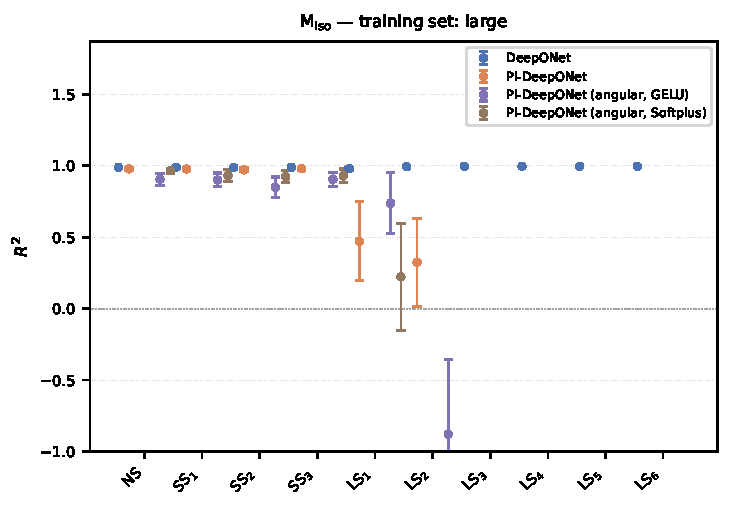
\includegraphics[width=\linewidth]{figures/R2_large.pdf}
    \caption{$R^2$ score.}
    \label{fig: R2 large}
\end{figure}

\begin{figure}
    \centering
    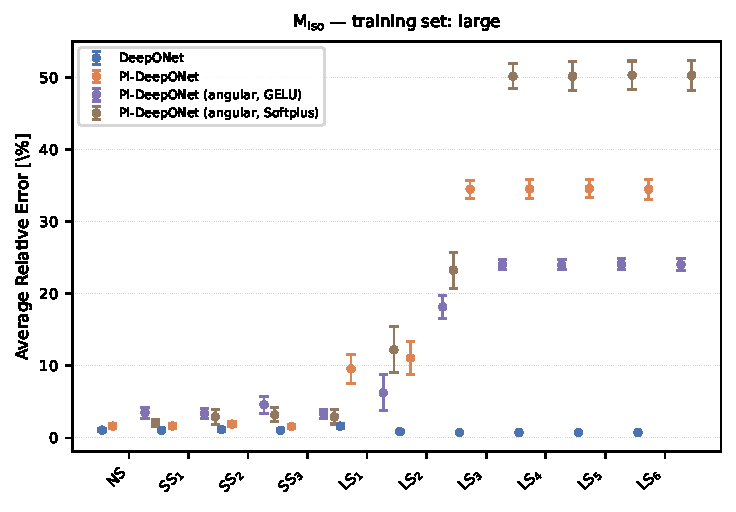
\includegraphics[width=\linewidth]{figures/ARE_large.pdf}
    \caption{ARE score.}
    \label{fig: ARE large}
\end{figure}

\section{Conclusion}

\bibliography{bibliography}

\end{document}